\documentclass[journal,12pt,onecolumn]{IEEEtran}
\usepackage{cite}
\usepackage{amsmath,amssymb,amsfonts,amsthm}
\usepackage{algorithmic}
\usepackage{graphicx}
\usepackage{textcomp}
\usepackage{xcolor}
\usepackage{txfonts}
\usepackage{listings}
\usepackage{circuitikz}
\usepackage{enumitem}
\usepackage{mathtools}
\usepackage{gensymb}
\usepackage{comment}
\usepackage[breaklinks=true]{hyperref}
\usepackage{tkz-euclide} 
\usepackage{gvv}                                        
\usepackage[latin1]{inputenc}                                
\usepackage{color}                                            
\usepackage{array}                                            
\usepackage{longtable}                                       
\usepackage{calc}                                             
\usepackage{multirow}                                         
\usepackage{hhline}                                           
\usepackage{ifthen}                                           
\usepackage{lscape}
\usepackage{tabularx}
\usepackage{array}
\usepackage{float}
\usepackage{multicol}
\usepackage{caption}
\usetikzlibrary{patterns}

\newtheorem{theorem}{Theorem}[section]
\newtheorem{problem}{Problem}
\newtheorem{proposition}{Proposition}[section]
\newtheorem{lemma}{Lemma}[section]
\newtheorem{corollary}[theorem]{Corollary}
\newtheorem{example}{Example}[section]
\newtheorem{definition}[problem]{Definition}
\newcommand{\BEQA}{\begin{eqnarray}}
\newcommand{\EEQA}{\end{eqnarray}}
\newcommand{\define}{\stackrel{\triangle}{=}}
\theoremstyle{remark}
\newtheorem{rem}{Remark}

% Marks the beginning of the document
\begin{document}
\bibliographystyle{IEEEtran}
\vspace{3cm}

\title{Assignment 12}
\author{DESABOINA SRI SATHWIK-AI24BTECH11007}
\maketitle
% Removed \newpage to avoid a blank first page
\bigskip

\section*{GATE-2024:EE}
\begin{enumerate}
    \item A 3-phase, $11\, kV$, $10\, MVA$ synchronous generator is connected to an inductive load of power factor $\frac{\sqrt{3}}{2}$ via a lossless line with a per-phase inductive reactance of $5 \,\ohm$. The per-phase synchronous reactance of the generator is $30\, \ohm$ with negligible armature resistance. If the generator is producing the rated current at the rated voltage, then the power factor at the terminal of the generator is
	   
	    \hfill{(EE:2024)}
		\begin{multicols}{4}
    \begin{enumerate}
        \item $0.63$ lagging.
        \item $0.87$ lagging.
        \item $0.63$ leading.
        \item $0.87$ leading.
    \end{enumerate}
\end{multicols}
    \item For the three-bus lossless power network shown in the figure, the voltage magnitudes at all the buses are equal to $1$ per unit ($pu$), and the differences of the voltage phase angles are very small. The line reactances are marked in the figure, where $\alpha$, $\beta$, $\gamma$, and $x$ are strictly positive. The bus injections $P_1$ and $P_2$ are in $pu$. If $P_1 = mP_2$, where $m > 0$, and the real power flow from bus $1$ to bus $2$ is $0\, pu$, then which one of the following options is correct?
\begin{figure}[!ht]
\centering

\begin{circuitikz}
\tikzstyle{every node}=[font=\small]

\draw (5,17.25) to[short] (5,15.25);
\draw (5,16.25) to[european resistor] (15.25,16.25);
\draw (15.25,17.25) to[short] (15.25,15.25);
\draw (5,15.75) to[short] (5.75,15.75);
\draw (15.25,15.75) to[short] (14.5,15.75);
\draw (5.75,15.75) to[european resistor] (9.5,12);
\draw (14.5,15.75) to[european resistor] (10.75,12);
\draw (9.5,12) to[short] (9.5,11.25);
\draw (10.75,12) to[short] (10.75,11.25);
\draw [ line width=0.8pt](8.75,11.25) to[short] (11.25,11.25);
\draw [line width=0.8pt, ->, >=Stealth] (3.5,16) -- (5,16);
\draw [line width=0.8pt, ->, >=Stealth] (17,16) -- (15.25,16);
\draw [line width=0.8pt, ->, >=Stealth] (10,11.25) -- (10,9.75);
\node [font=\normalsize] at (16.5,16.25) {$P_2$};
\node [font=\normalsize] at (3.75,16.25) {$P_1$};
\node [font=\normalsize] at (5.75,16.5) {bus $1$};
\node [font=\normalsize] at (14.5,16.5) {bus $2$};
\node [font=\normalsize] at (11.5,12) {bus $3$};
\node [font=\small] at (10,15.75) {$j\alpha x\, \ohm$};
\node [font=\small] at (6.5,13.75) {$j\beta x\, \ohm$};
\node [font=\small] at (13.5,13.5) {$j\gamma x\, \ohm$};
\end{circuitikz}

\end{figure}

	    
	    \hfill{(EE:2024)}
		\begin{multicols}{4}
    \begin{enumerate}
        \item $\gamma = m\beta$
        \item $\beta = m\gamma$
        \item $\alpha = m\gamma$
        \item $\alpha = m\beta$
    \end{enumerate}
			\end{multicols}

    \item A BJT biasing circuit is shown in the figure, where $V_{BE} = 0.7\, V$ and $\beta = 100$. The Quiescent Point values of $V_{CE}$ and $I_C$ are respectively 
	    \begin{figure}[!ht]
\centering
\begin{circuitikz}
\tikzstyle{every node}=[font=\normalsize]
\draw [ line width=0.8pt](7,16.75) to[R] (7,13.5);
\draw [ line width=0.8pt](7,13.5) to[R] (7,9.25);
\draw [ line width=0.8pt](7,16.75) to[short] (10.5,16.75);
\draw [ line width=0.8pt](7,9.25) to[short] (10.5,9.25);
\draw [ line width=0.8pt](10.5,9.25) to[R] (10.5,12.75);
\draw [ line width=0.8pt](10.5,13.25) to[R] (10.5,16.75);
\draw [ line width=0.8pt](7,13) to[short] (9.75,13);
\draw [ line width=0.8pt](9.75,13.5) to[short] (9.75,12.5);
\draw [ line width=0.8pt](9.75,13) to[short] (7,13);
\draw [ line width=0.8pt](9.75,13.25) to[short] (10.5,13.25);
\draw [ line width=0.8pt](9.75,12.75) to[short] (10.5,12.75);
\draw [line width=0.8pt, ->, >=Stealth] (10.5,14.25) -- (10.5,13.75);
\draw [line width=0.8pt, ->, >=Stealth] (10,12.75) -- (10.25,12.75);
\draw [line width=0.8pt, ->, >=Stealth] (10.5,16.75) -- (10.5,17.5);
\draw [line width=0.8pt](10.5,9.25) to (10.5,9) node[ground]{};
\node [font=\normalsize] at (5.25,15.25) {$R_1 = 100\, k\ohm$};
\node [font=\normalsize] at (5.25,11.25) {$R_2 = 50\, k\ohm$};
\node [font=\normalsize] at (12,15) {$R_C = 2\, k\ohm$};
\node [font=\normalsize] at (12,11) {$R_E = 1\, k\ohm$};
\node [font=\small] at (10.75,13.25) {$+$};
\node [font=\small] at (10.75,12.75) {$-$};
\node [font=\normalsize] at (11.5,13) {$V_{CE}$};
\node [font=\normalsize] at (10.75,18) {$V_{CC} = +12V$};
\node [font=\normalsize] at (10,14) {$I_C$};
\node [font=\normalsize] at (13.5,16.25) {$Text$};
\end{circuitikz}

\label{fig:my_label}
\end{figure}

	   
	    \hfill{(EE:2024)}
		\begin{multicols}{2}
    \begin{enumerate}
        \item $4.6\, V$ and $2.46\, mA$
        \item $3.5\, V$ and $2.46\, mA$
        \item $2.61\, V$ and $3.13\, mA$
        \item $4.6\, V$ and $3.13\, mA$
    \end{enumerate}
			\end{multicols}

    \item Let $f(t)$ be a real-valued function whose second derivative is positive for $-\infty < t < \infty$. Which of the following statements is/are always true?
	  
	    \hfill{(EE:2024)}

    \begin{enumerate}
        \item $f(t)$ has at least one local minimum.
        \item $f(t)$ cannot have two distinct local minima.
        \item $f(t)$ has at least one local maximum.
        \item The minimum value of $f(t)$ cannot be negative.
    \end{enumerate}

    \item Consider the function $f(t) = (\max(0, t))^2$ for $-\infty < t < \infty$, where $\max(a, b)$ denotes the maximum of $a$ and $b$. Which of the following statements is/are true? 

	    \hfill{(EE:2024)}
    \begin{enumerate}
        \item $f(t)$ is not differentiable.
        \item $f(t)$ is differentiable and its derivative is continuous.
        \item $f(t)$ is differentiable but its derivative is not continuous.
        \item $f(t)$ and its derivative are differentiable.
    \end{enumerate}

    \item Which of the following differential equations is/are nonlinear? 

	    \hfill{(EE:2024)}
		\begin{multicols}{2}
    \begin{enumerate}
        \item $t x(t) + \frac{dx(t)}{dt} = t^2 e^t, \quad x(0) = 0$
        \item $\frac{1}{2} e^t + x(t) \frac{dx(t)}{dt} = 0, \quad x(0) = 0$
        \item $x(t) \cos t - \frac{dx(t)}{dt} \sin t = 1, \quad x(0) = 0$
        \item $x(t) + e^{\left(\frac{dx(t)}{dt}\right)} = 1, \quad x(0) = 0$
    \end{enumerate}
			\end{multicols}

    \item For a two-phase network, the phase voltages $V_p$ and $V_q$ are to be expressed in terms of sequence voltages $V_\alpha$ and $V_\beta$ as $\myvec{ V_p \\ V_q } = S \myvec{ V_\alpha \\ V_\beta }$. The possible option(s) for matrix $S$ is/are 

		    \hfill{(EE:2024)}
		    \begin{multicols}{4}
    \begin{enumerate}
        \item $\myvec{ 1 & 1 \\ 1 & -1 }$
        \item $\myvec{ 1 & 1 \\ 1 & 1 }$
        \item $\myvec{ 1 & 1 \\ 1 & 0 }$
        \item $\myvec{ -1 & 1 \\ 1 & 1 }$
    \end{enumerate}
			    \end{multicols}

    \item Which of the following options is/are correct for the Automatic Generation Control (AGC) and Automatic Voltage Regulator (AVR) installed with synchronous generators?

	    \hfill{(EE:2024)}
    \begin{enumerate}
        \item AGC response has a local effect on frequency while AVR response has a global effect on voltage.
        \item AGC response has a global effect on frequency while AVR response has a local effect on voltage.
        \item AGC regulates the field current of the synchronous generator while AVR regulates the generator's mechanical power input.
        \item AGC regulates the generator's mechanical power input while AVR regulates the field current of the synchronous generator.
    \end{enumerate}

    \item Two passive two-port networks \textbf{P} and \textbf{Q} are connected as shown in the figure. The impedance matrix of network \textbf{P} is $Z_P = \myvec{ 40 \Omega & 60 \Omega \\ 80 \Omega & 100 \Omega }$. The admittance matrix of network \textbf{Q} is $Y_Q = \myvec{ 5\, S & -2.5\, S \\ -2.5\, S & 1\, S}$. Let the ABCD matrix of the two-port network \textbf{R} in the figure be $\myvec{ \alpha & \beta \\ \gamma & \delta }$. The value of $\beta$ in $\Omega$ is \rule{2.5cm}{0.4pt} (rounded off to 2 decimal places).
	    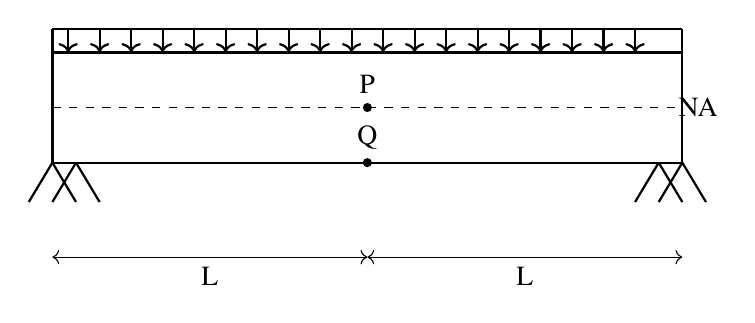
\begin{tikzpicture}

    % Beam
    \draw[thick] (-4,0) -- (4,0);
 \draw[thick] (-4,1.4) -- (4,1.4);
 \draw[thick] (-4,1.7) -- (4,1.7);
 \draw[thick] (-4,0) -- (-4,1.7);
 \draw[thick] (4,0) -- (4,1.7);


    % Supports
    \draw[thick] (-4,-0.5) -- (-3.7,0);
    \draw[thick] (-4.3,-0.5) -- (-4,0);
    \draw[thick] (4,-0.5) -- (3.7,0);
    \draw[thick] (4.3,-0.5) -- (4,0);
    \draw[thick] (3.7,-0.5) -- (4,0);
    \draw[thick] (3.4,-0.5) -- (3.7,0);
	\draw[thick] (-3.7,-0.5) -- (-4,0);
	\draw[thick] (-3.4,-0.5) -- (-3.7,0);

    % Distributed load
    \foreach \x in {-3.8,-3.4,...,3.8}
        \draw[thick,->] (\x,1.7) -- (\x,1.4);

    % Neutral Axis
    \draw[dashed] (-4,0.7) -- (4,0.7);
    \node at (4.2,0.7) {NA};

    % Points P and Q
    \draw[fill=black] (0,0.7) circle (0.05);
    \node[above] at (0,0.75) {P};
    \draw[fill=black] (0,0) circle (0.05);
    \node[above] at (0,0.05) {Q};

    % Dimensions
    \draw[<->] (-4,-1.2) -- (0,-1.2);
    \node[below] at (-2,-1.2) {L};
    \draw[<->] (0,-1.2) -- (4,-1.2);
    \node[below] at (2,-1.2) {L};

\end{tikzpicture}



		    \hfill{(EE:2024)}

    \item For the circuit shown in the figure, the source frequency is $5000 \, rad/sec$. The mutual inductance between the magnetically coupled inductors is 5 mH with their self inductances being $125\, mH$ and $1\, mH$. The Thevenin's impedance, $Z_{th}$, between the terminals $P$ and $Q$ in $\ohm$ is  \rule{2cm}{0.4pt} (rounded off to 2 decimal places). 
	    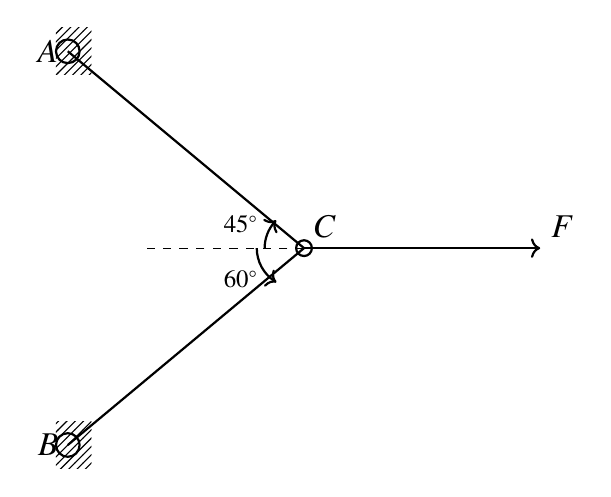
\begin{tikzpicture}
    % Define points with A and B further left and spaced vertically
    \coordinate (A) at (-3,2.5);
    \coordinate (B) at (-3,-2.5);
    \coordinate (C) at (0,0);
    \coordinate (F) at (3,0);

    % Draw fixed supports at A and B
    \fill[pattern=north east lines] (-3.15,2.8) rectangle (-2.7,2.2);
    \fill[pattern=north east lines] (-3.15,-2.2) rectangle (-2.7,-2.8);
    
    % Draw circles at supports
    \draw[thick] (A) circle(0.15);
    \draw[thick] (B) circle(0.15);
    \draw[thick] (C) circle(0.1);

    % Draw the rods AC and BC
    \draw[thick] (A) -- (C);
    \draw[thick] (B) -- (C);

    % Draw force arrow at C and label at the end
    \draw[thick, ->] (C) -- (F) node[above right] {\large $F$};

    % Draw a dashed line from C to the left
    \draw[dashed] (C) -- ++(-2,0);

    % Draw angle arcs and labels in correct positions
    \draw[thick, ->] (-0.5,0) arc[start angle=180, end angle=135, radius=0.5];
    \node at (-0.8,0.3) {\small $45^\circ$};
    
    \draw[thick, ->] (-0.6,0) arc[start angle=180, end angle=240, radius=0.5];
    \node at (-0.8,-0.4) {\small $60^\circ$};

    % Label points A, B, and C
    \node[left] at (A) {\large $A$};
    \node[left] at (B) {\large $B$};
    \node[above right] at (C) {\large $C$};

\end{tikzpicture}


	    \hfill{(EE:2024)}

    \item In the circuit shown, $Z_1 = 50\angle -90^\circ \, \ohm$ and $Z_2 = 200\angle -30^\circ \, \ohm$. It is supplied by a three phase $400\, V$ source with the phase sequence being R-Y-B. Assume the watt meters $W_1$ and $W_2$ to be ideal. The magnitude of the difference between the readings of $W_1$ and $W_2$ in watts is \rule{2.5cm}{0.4pt} (rounded off to 2 decimal places).
	    \begin{tikzpicture}
    % Draw the x and y axes
    \draw[->] (-1.5, 0) -- (1.5, 0) node[right] {$x$};
    \draw[->] (0, -1.5) -- (0, 1.5) node[above] {$y$};
    
    % Draw the optic axis at 135° angle
    \draw[dashed, ->] (1.2, -1.2) -- (-1.2, 1.2);
    \node at (-2, 1) {Optic axis};

    
    % Draw the 135° angle arc
    \draw[->] (0.5, 0) arc[start angle=0, end angle=135, radius=0.5];
    \node at (0.8, 0.3) {$135^\circ$};
\end{tikzpicture}



	    \hfill{(EE:2024)}

    \item In the $(x, y, z)$ coordinate system, three point-charges $Q$, $Q$, and $\alpha Q$ are located in free space at $(-1, 0, 0)$, $(1, 0, 0)$, and $(0, -1, 0)$, respectively. The value of $\alpha$ for the electric field to be zero at $(0, 0.5, 0)$ is \rule{2.5cm}{0.4pt} (rounded off to 1 decimal place). 

	    \hfill{(EE:2024)}

    \item The given equation represents a magnetic field strength $\vec{H}(r, \theta, \phi)$ in the spherical coordinate system, in free space. Here, $\hat{r}$ and $\theta$ represent the unit vectors along $r$ and $\theta$, respectively. The value of $P$ in the equation should be  \rule{2.5cm}{0.4pt} (rounded off to the nearest integer).\\
	    \begin{center}
$\overline{H}(r, \theta, \phi) = \frac{1}{r^3} \left( \hat{r} P \cos \theta + \hat{\theta} \sin \theta \right)$
	    \end{center}

	    \hfill{(EE:2024)}
\end{enumerate}
\end{document}
